\chapter{閉弦、能階匹配與對偶性}

\lectureoverview{閉弦沿著兩個內在方向各自承載獨立的波。將這些波量子化，乍看之下似乎會使開弦的光子數加倍，但弦座標原點平移下的不變性會排除只存在於單一方向的狀態。第一個留下的能階含有一個無質量自旋二粒子。改變描述方式的同一個想法，接著引出一個更廣泛的問題：耦合變化時，稱任何物件為基本的究竟有什麼意義？}

\section{留待後用的生成元}

在畫出閉弦之前，先回顧一個正則力學的結果。設
\begin{equation}
  L=L(q_i,\dot q_i),
\end{equation}
並將與 \(q_i\) 共軛的動量定義為
\begin{equation}
  p_i=\frac{\partial L}{\partial\dot q_i}.
\end{equation}
無窮小連續變換可寫成
\begin{equation}
  \delta q_i=\epsilon f_i(q),
  \label{eq:l04-infinitesimal-transformation}
\end{equation}
其中 \(\epsilon\) 是一個小參數。若此變換是對稱性，諾特定理便會給出守恆荷。將座標位移除以共同參數，就得到生成元
\begin{equation}
  Q=\sum_i p_i f_i(q)
   =\frac{1}{\epsilon}\sum_i p_i\,\delta q_i.
  \label{eq:l04-noether-charge}
\end{equation}
在量子力學中，\(Q\) 是生成相應無窮小變換的算符。

在 \(xy\) 平面上的旋轉是個熟悉的例子。採用其中一種取向約定，
\begin{equation}
  \delta x=\epsilon y,
  \qquad
  \delta y=-\epsilon x,
\end{equation}
而 \eqref{eq:l04-noether-charge} 就是角動量，至多差一個相同的符號約定。這個具體例子並不重要；重要的是其一般形式：動量與無窮小位移縮並，便得到生成元。

\begin{figure}[H]
  \centering
  \includegraphics[width=0.76\textwidth]{lecture_04_figure_01.png}
  \caption{為稍後平移閉弦座標時保留的正則動量與諾特生成元。}
  \lectureframe{00:05:00}
  \label{fig:l04-noether-board}
\end{figure}

我們很快會遇到一種對稱性，其座標不是普通空間中的點，而是弦上各點的標記。式 \eqref{eq:l04-noether-charge} 正是為此預先備妥的。

\section{環繞一圈的座標}

閉弦沒有端點。選取一個參數
\begin{equation}
  0\leq \sigma<2\pi
\end{equation}
並暫時將其中一點標記為 \(\sigma=0\)。繞行半圈的位置是 \(\sigma=\pi\)；四分之一圈與四分之三圈的位置分別是 \(\pi/2\) 和 \(3\pi/2\)。這個標記建立的是座標約定，尚非物理特徵。

\begin{figure}[H]
  \centering
  \begin{minipage}[t]{0.58\textwidth}
    \centering
    \includegraphics[width=\textwidth]{lecture_04_figure_02.png}
    \par\smallskip\footnotesize (a) 黑板上標出記號的圈。
  \end{minipage}\hfill
  \begin{minipage}[t]{0.37\textwidth}
    \centering
    \begin{adjustbox}{max width=\linewidth}
    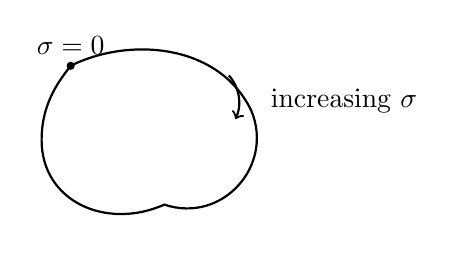
\begin{tikzpicture}[scale=0.82]
      \draw[thick]
        (0.1,1.1)
        .. controls (1.0,1.55) and (2.4,1.45) .. (2.9,0.4)
        .. controls (3.25,-0.45) and (2.45,-1.35) .. (1.55,-1.05)
        .. controls (0.65,-1.45) and (-0.35,-1.0) .. (-0.35,-0.05)
        .. controls (-0.35,0.55) and (-0.05,0.9) .. (0.1,1.1);
      \fill (0.1,1.1) circle (1.8pt);
      \node[above] at (0.1,1.12) {\(\sigma=0\)};
      \draw[->,thick] (2.55,0.95) arc[start angle=42,end angle=-25,radius=0.62];
      \node[right] at (3.05,0.55) {increasing \(\sigma\)};
    \end{tikzpicture}
    \end{adjustbox}
    \par\smallskip\footnotesize (b) 內在取向。
  \end{minipage}
  \caption{標記一點以定義原點，並以箭頭標示 \(\sigma\) 增大的方向。}
  \lectureframe{00:06:48}
  \label{fig:l04-closed-string-origin}
\end{figure}

沿著圈的箭頭表示一種\emph{內在}取向。不可將它與 \(xy\) 平面上的順時針或逆時針運動混為一談。想像將一條標了記號的橡皮筋從黑板上拿起、翻面，再放回去。它表面上的順時針方向會反轉，但內在記號的排列順序不變。\(\sigma\) 增大的方向仍然是 \(\sigma\) 增大的方向。

這項區分決定了右行波與左行波的用法。在本章中，右行擾動指沿著 \(\sigma\) 增大的方向傳播的擾動，左行擾動則指沿著 \(\sigma\) 減小的方向傳播的擾動。這兩個名稱都不表示擾動在房間裡看起來朝哪個方向移動。

在早期強子弦圖像中，取向曾扮演具體角色。將一條有取向的通量管斷開，會在一端產生夸克，在另一端產生反夸克；內在箭頭可區分這兩端。也可以建構無取向的弦理論，但在此處的討論中，我們保留箭頭以及沿箭頭的兩個方向。

\section{週期性與行波}

令 \(X(\sigma,\tau)\) 和 \(Y(\sigma,\tau)\) 為弦的兩個橫向座標，並以 \(\tau\) 表示時間。若還有其他橫向座標，處理方式也完全相同。由於 \(\sigma=0\) 和 \(\sigma=2\pi\) 標記的是同一點，
\begin{equation}
  X(\sigma+2\pi,\tau)=X(\sigma,\tau),
  \qquad
  Y(\sigma+2\pi,\tau)=Y(\sigma,\tau).
  \label{eq:l04-periodicity}
\end{equation}

\begin{figure}[H]
  \centering
  \includegraphics[width=0.76\textwidth]{lecture_04_figure_03.png}
  \caption{兩個橫向座標的週期性邊界條件。}
  \lectureframe{00:12:40}
  \label{fig:l04-periodicity-board}
\end{figure}

因此，局部擾動可以不斷繞圈傳播。抵達 \(2\pi\) 時，它會直接在 \(0\) 再度出現。這與開弦不同：行波抵達端點後會反射，原本左行的波變成右行，反之亦然。駐波適用於開弦，而閉弦則容許兩個彼此獨立傳播的波族。

\subsection{複數傅立葉模態}

週期函數的一組方便基底是
\begin{equation}
  e^{in\sigma}=\cos(n\sigma)+i\sin(n\sigma),
  \qquad n\in\mathbb Z.
\end{equation}
週期性要求指標為整數：
\(e^{in(\sigma+2\pi)}=e^{in\sigma}\)。例如，若將 \(n\) 換成半整數，函數在繞行一圈後就會改變。

暫時略去時間依賴後，黑板上的展開式為
\begin{align}
  X(\sigma)
  &=
  X_0+
  \sum_{n>0}X_n e^{in\sigma}
  +\sum_{n>0}X_{-n}e^{-in\sigma},
  \label{eq:l04-fourier-x}\\
  Y(\sigma)
  &=
  Y_0+
  \sum_{n>0}Y_n e^{in\sigma}
  +\sum_{n>0}Y_{-n}e^{-in\sigma}.
  \label{eq:l04-fourier-y}
\end{align}
在經典層次上，若 \(X\) 和 \(Y\) 為實數，負指標的係數便是相應正指標係數的複共軛。零模 \(X_0\) 和 \(Y_0\) 指定質心的位置；它們是位置，不是內部振動。

\begin{figure}[H]
  \centering
  \includegraphics[width=0.82\textwidth]{lecture_04_figure_04.png}
  \caption{週期傅立葉展開中正指標與負指標的部分，以及零模。}
  \lectureframe{00:20:00}
  \label{fig:l04-fourier-board}
\end{figure}

\begin{classroomqa}
\audiencequestion{如果這些是行波，時間座標在哪裡？\lecturetimestamp{00:19:05}}
\lecturerresponse{它只是在黑板記號中暫時省略了。行波解的相位同時包含 \(\sigma\) 和 \(\tau\)。採用下文的約定，其中一個波族的相位是
\(e^{-in(\tau-\sigma)}\)，另一個則是
\(e^{-in(\tau+\sigma)}\)。}
\end{classroomqa}

因此，決定傳播方向的是完整相位，而不是單看純空間傅立葉因子中 \(n\) 的正負號。我們可以寫成
\begin{equation}
  X(\sigma,\tau)=X_R(\tau-\sigma)+X_L(\tau+\sigma),
  \label{eq:l04-chiral-solution}
\end{equation}
對 \(Y\) 也可作同樣表示。將哪一族稱為 \(R\)、哪一族稱為 \(L\)，只是約定；不變的事實是，沿著 \(\sigma\) 圓有兩個相反的方向。\editorialnote{\(e^{in\sigma}\) 這個因子在某一瞬間本身並不足以指定行波。必須給定時間相位，才能確定傳播方向。}

\section{兩個方向上的能量}

局部動力學與開弦相同。在此採用的簡化歸一化下，
\begin{equation}
  L\propto
  \int_0^{2\pi}d\sigma\,
  \left[
    \dot X^2-X'^2+\dot Y^2-Y'^2
  \right],
  \label{eq:l04-string-lagrangian}
\end{equation}
其中點號表示 \(\partial_\tau\)，撇號表示 \(\partial_\sigma\)。動能項與彈性項在能量中以正號相加：
\begin{equation}
  E\propto
  \int_0^{2\pi}d\sigma\,
  \left[
    \dot X^2+X'^2+\dot Y^2+Y'^2
  \right].
  \label{eq:l04-string-energy}
\end{equation}
對任一橫向座標，
\begin{equation}
  \dot X^2+X'^2
  =
  \frac12(\dot X+X')^2+
  \frac12(\dot X-X')^2.
  \label{eq:l04-energy-square-completion}
\end{equation}
交叉項會相消，恰好留下原有的動能與梯度能。

\begin{figure}[H]
  \centering
  \includegraphics[width=0.82\textwidth]{lecture_04_figure_05.png}
  \caption{總能量重新整理為兩個行波扇區的能量。}
  \lectureframe{00:25:10}
  \label{fig:l04-energy-board}
\end{figure}

對 \(X_R(\tau-\sigma)\)，有 \(\dot X_R=-X_R'\)；對 \(X_L(\tau+\sigma)\)，則有 \(\dot X_L=X_L'\)。因此，\eqref{eq:l04-energy-square-completion} 中的兩個平方項分別挑出兩個手徵波族。將所有橫向座標都納入，定義
\begin{align}
  E_L&\propto
  \frac12\int_0^{2\pi}d\sigma
  \sum_I(\dot X^I+X^{I\prime})^2,\\
  E_R&\propto
  \frac12\int_0^{2\pi}d\sigma
  \sum_I(\dot X^I-X^{I\prime})^2.
  \label{eq:l04-left-right-energies}
\end{align}
於是 \(E=E_L+E_R\)。此時方程是線性的，因此兩個扇區的波會彼此交錯通過而不發生散射。

\subsection{振子數加倍}

將傅立葉級數代入 \eqref{eq:l04-string-lagrangian}，每個非零模態係數都會成為一個諧振子。其頻率正比於 \(|n|\)：波長越短，頻率越高，激發能也越大。不同於開弦，每個正頻率都有兩個獨立傳播的副本。

黑板上將 \(X\) 極化的產生算符標記為 \(a_n^+\) 和 \(a_{-n}^+\)，將 \(Y\) 極化的產生算符標記為 \(b_n^+\) 和 \(b_{-n}^+\)。為了更清楚地區分產生算符與傳播方向，我們採用記號
\begin{equation}
  a_n^\dagger,\quad b_n^\dagger,
  \qquad
  \widetilde a_n^\dagger,\quad\widetilde b_n^\dagger,
  \qquad n>0.
  \label{eq:l04-oscillator-notation}
\end{equation}
不帶波浪號與帶波浪號的算符分別產生沿世界面相反方向傳播的振子；\(a\) 和 \(b\) 表示兩個橫向極化。

\begin{figure}[H]
  \centering
  \includegraphics[width=0.65\textwidth]{lecture_04_figure_06.png}
  \caption{黑板上 \(X\) 與 \(Y\) 極化所對應的兩組產生算符。}
  \lectureframe{00:29:10}
  \label{fig:l04-oscillators-board}
\end{figure}

若 \(N_n^{(a)},N_n^{(b)}\) 及其帶波浪號的對應量表示佔據數，則兩個方向上的振子能階可概略寫成
\begin{equation}
  \begin{aligned}
    N&=\sum_{n>0}n\bigl(N_n^{(a)}+N_n^{(b)}+\cdots\bigr),\\
    \widetilde N&=\sum_{n>0}n
      \bigl(\widetilde N_n^{(a)}+\widetilde N_n^{(b)}+\cdots\bigr).
  \end{aligned}
  \label{eq:l04-level-operators}
\end{equation}
省略號代表其他橫向方向。

\section{錯誤的譜猜測}

回顧開弦的第一能階。以 \(a_1^\dagger\) 或 \(b_1^\dagger\) 作用於基態，會得到兩個線偏振。它們的圓偏振組合為
\begin{equation}
  c_\pm^\dagger
  =
  \frac{1}{\sqrt2}
  \left(a_1^\dagger\pm i b_1^\dagger\right),
  \label{eq:l04-open-circular}
\end{equation}
具有螺旋度 \(h=\pm1\)。沒有螺旋度為零的夥伴，正是這個初階四維描述中無質量向量粒子的特徵。

令閉弦基態的質量平方為 \(m_0^2\)。一個初步而天真的猜測是，從下列算符中任選一個作用一次：
\begin{equation}
  a_1^\dagger,\quad b_1^\dagger,\quad
  \widetilde a_1^\dagger,\quad\widetilde b_1^\dagger.
  \label{eq:l04-naive-one-sided}
\end{equation}
這看起來像是開弦光子的兩個副本，分別對應兩個傳播方向。然而到了下一個能量，這份不受限制的清單無法組成合理的轉動多重態。更複雜的整理方式也無法解決問題。錯的是「每個振子單項式都是物理態」這項假設。

\subsection{先將能階匹配視為規則}

閉弦的物理條件是
\begin{equation}
  N=\widetilde N,
  \qquad\text{equivalently}\qquad E_L=E_R.
  \label{eq:l04-level-matching}
\end{equation}
目前先將它視為假設；等看過它能達成什麼效果後，再推導其由來。

\eqref{eq:l04-naive-one-sided} 中的每個狀態都只在一個扇區有一單位的能量，另一扇區則沒有，因此全都被排除。最先留下的狀態在每個波族中各帶有一個振子：
\begin{align}
  a_1^\dagger\widetilde a_1^\dagger\ket{0},
  &\qquad
  b_1^\dagger\widetilde b_1^\dagger\ket{0},
  \label{eq:l04-four-matched-a}\\
  a_1^\dagger\widetilde b_1^\dagger\ket{0},
  &\qquad
  b_1^\dagger\widetilde a_1^\dagger\ket{0}.
  \label{eq:l04-four-matched-b}
\end{align}
它們的振子總能量為二，平均分配在兩個方向上。單一 \(n=2\) 產生算符的振子總能量也相同，但不符合 \eqref{eq:l04-level-matching}；它只在其中一側貢獻兩個能量單位。

\begin{figure}[H]
  \centering
  \includegraphics[width=0.70\textwidth]{lecture_04_figure_07.png}
  \caption{通過能階匹配的第一能階四個狀態。圖中使用下標 \(1\) 和 \(-1\)；而 \eqref{eq:l04-four-matched-a}--\eqref{eq:l04-four-matched-b} 則使用不帶波浪號與帶波浪號的算符。}
  \lectureframe{00:41:05}
  \label{fig:l04-level-matched-board}
\end{figure}

\section{第一個匹配能階中的引力子}

將兩個手徵波族都改用圓偏振基底表示：
\begin{equation}
  c_\pm^\dagger
  =\frac{a_1^\dagger\pm i b_1^\dagger}{\sqrt2},
  \qquad
  \widetilde c_\pm^\dagger
  =\frac{\widetilde a_1^\dagger\pm i\widetilde b_1^\dagger}{\sqrt2}.
  \label{eq:l04-closed-circular}
\end{equation}
在一般的橫向空間中，每個因子各自貢獻螺旋度 \(+1\) 或 \(-1\)。因此，兩者的乘積為
\begin{center}
\begin{tabular}{c c}
  \toprule
  狀態 &螺旋度 \\
  \midrule
  \(c_+^\dagger\widetilde c_+^\dagger\ket0\) & \(+2\) \\
  \(c_-^\dagger\widetilde c_-^\dagger\ket0\) & \(-2\) \\
  \(c_+^\dagger\widetilde c_-^\dagger\ket0\) & \(0\) \\
  \(c_-^\dagger\widetilde c_+^\dagger\ket0\) & \(0\) \\
  \bottomrule
\end{tabular}
\end{center}

\begin{classroomqa}
\audiencequestion{第二個圓偏振因子是否應該來自相反的傳播扇區？\lecturetimestamp{00:43:20}}
\lecturerresponse{是的。黑板上最初寫下的表示式，正是基於這個原因而更正的。此處的物理態必須將一個右行振子與一個左行振子配成一對，否則就不符合能階匹配。螺旋度指的是橫向空間中的極化，而兩個因子則分別對應世界面的相反方向。}
\end{classroomqa}

\begin{figure}[H]
  \centering
  \includegraphics[width=0.82\textwidth]{lecture_04_figure_08.png}
  \caption{黑板更正後的四個圓偏振基底乘積，其螺旋度為 \(+2,-2,0,0\)。}
  \lectureframe{00:46:10}
  \label{fig:l04-helicity-board}
\end{figure}

有質量的自旋二粒子有五種自旋投影：
\begin{equation}
  m=2,1,0,-1,-2.
\end{equation}
匹配能階中沒有 \(m=\pm1\) 的夥伴，因此不可能構成有質量的自旋二多重態。相較之下，無質量自旋二粒子只有螺旋度 \(+2\) 和 \(-2\)。同螺旋度的乘積恰好就是這兩個狀態：它們是引力子的兩種極化。

還有兩個螺旋度為零的組合。在課堂所用的說法中，一個是膨脹子，另一個是軸子。一般閉弦玻色弦的協變描述則將這項說法進一步細分：
\begin{equation}
  \begin{aligned}
    \alpha_{-1}^{I}\widetilde\alpha_{-1}^{J}\ket{0;k}
    &\longrightarrow
    \underbrace{h_{IJ}}_{\text{symmetric traceless}}
    \oplus
    \underbrace{B_{IJ}}_{\text{antisymmetric}}\\
    &\hspace{2.5em}\oplus
    \underbrace{\Phi}_{\text{trace}}.
  \end{aligned}
  \label{eq:l04-massless-tensor-decomposition}
\end{equation}
這些場分別是引力子、反對稱二形式場與膨脹子。在四維中，二形式場可對偶化為類軸子的贗純量，這就是講課採用的說法。\editorialnote{第二個螺旋度為零的狀態，在一般閉弦譜中從根本上說是反對稱張量場 \(B_{\mu\nu}\)。稱它為軸子，指的是其在四維中的對偶描述。}

在這個形式層次上，三個場都是無質量的。緊緻化、投影與背景動力學可能改變哪些純量或二形式自由度仍然是輕的。引力子則不同：只要存在自洽且相互作用的閉弦扇區，無質量自旋二狀態便不可避免。因此，引力是從閉弦中浮現，而非另行加入的成分。

\section{為何能階必須匹配}

現在回到 \(\sigma=0\) 處的標記。它是固定在圈上的實體珠子，還是僅僅代表參數的原點？對於沒有標記的普通閉弦，不應有任何一點受到特殊對待。所有標記一起平移時，量子態必須保持不變。

\subsection{離散版本}

將圈離散化為 \(M\) 個依序排列的點，其橫向座標為 \((X_i,Y_i)\)。暫時略去 \(Y_i\)。位形空間中的波函數寫作
\begin{equation}
  \Psi(X_1,X_2,\ldots,X_M).
\end{equation}
改變哪個點被視為第一個點，會形成循環置換：
\begin{align}
  \Psi(X_1,X_2,\ldots,X_M)
  &=
  \Psi(X_2,\ldots,X_M,X_1)\nonumber\\
  &=
  \Psi(X_3,\ldots,X_M,X_1,X_2).
  \label{eq:l04-cyclic-wavefunction}
\end{align}
這並不表示波函數在任意置換下都不變。例如，在 \(X_1\) 和 \(X_2\) 之間插入 \(X_3\)，會改變相鄰關係，等同於撕開並重新接合離散化的弦。只有共同的循環重標記
\begin{equation}
  X_i\longrightarrow X_{i+1}\qquad(\text{mod }M)
  \label{eq:l04-discrete-shift}
\end{equation}
才能表達不存在優先原點。

\begin{figure}[H]
  \centering
  \includegraphics[width=0.82\textwidth]{lecture_04_figure_09.png}
  \caption{離散化閉弦的循環波函數關係式。}
  \lectureframe{00:56:20}
  \label{fig:l04-cyclic-board}
\end{figure}

\subsection{連續版本}

在連續極限 \(M\to\infty\) 下，狀態由波泛函表示：
\begin{equation*}
  \Psi[X(\sigma),Y(\sigma)].
\end{equation*}
循環重標記對應為
\begin{equation}
  \sigma\longrightarrow\sigma+\epsilon.
\end{equation}
不變性表示
\begin{equation}
  \Psi[X(\sigma+\epsilon),Y(\sigma+\epsilon)]
  =
  \Psi[X(\sigma),Y(\sigma)].
  \label{eq:l04-wavefunctional-invariance}
\end{equation}

\begin{figure}[H]
  \centering
  \includegraphics[width=0.72\textwidth]{lecture_04_figure_10.png}
  \caption{離散平移及其波泛函形式的連續極限。}
  \lectureframe{00:58:40}
  \label{fig:l04-wavefunctional-board}
\end{figure}

在一階近似下，
\begin{equation}
  \delta X(\sigma)=\epsilon X'(\sigma),
  \qquad
  \delta Y(\sigma)=\epsilon Y'(\sigma),
  \label{eq:l04-profile-shift}
\end{equation}
整體正負號取決於我們要區分的是對剖面作主動平移，還是對座標作被動平移。相應的波泛函變分為
\begin{equation}
  \delta\Psi
  =
  \epsilon\int_0^{2\pi}d\sigma
  \left[
    \frac{\delta\Psi}{\delta X(\sigma)}X'(\sigma)
    +
    \frac{\delta\Psi}{\delta Y(\sigma)}Y'(\sigma)
  \right].
  \label{eq:l04-functional-variation}
\end{equation}

\begin{figure}[H]
  \centering
  \includegraphics[width=0.72\textwidth]{lecture_04_figure_11.png}
  \caption{平移後波泛函自變數的一階展開。}
  \lectureframe{01:01:31}
  \label{fig:l04-functional-expansion-board}
\end{figure}

\begin{classroomqa}
\audiencequestion{一階條件是否對 \(\sigma\) 的每個值各自構成一條獨立方程？\lecturetimestamp{01:01:30}}
\lecturerresponse{不是。此變換會一併平移弦上的所有點。某一點的變分必須與其餘各點的變分相加，因此連續形式中才會出現對 \(\sigma\) 的積分。}
\end{classroomqa}

在座標表象中，
\begin{equation}
  P_X(\sigma)=-i\frac{\delta}{\delta X(\sigma)},
  \qquad
  P_Y(\sigma)=-i\frac{\delta}{\delta Y(\sigma)}
  \label{eq:l04-functional-momenta}
\end{equation}
其中 \(\hbar=1\)。因此，方程 \eqref{eq:l04-functional-variation} 是由下列生成元所生成：
\begin{equation}
  G_\sigma=
  \int_0^{2\pi}d\sigma\,
  \left[
    P_X(\sigma)X'(\sigma)+P_Y(\sigma)Y'(\sigma)
  \right].
  \label{eq:l04-sigma-generator}
\end{equation}
這正是諾特定理的一般形式 \eqref{eq:l04-noether-charge}：將正則動量乘上座標位移，並對所有自由度加總。無標記的閉弦狀態滿足
\begin{equation}
  G_\sigma\ket{\mathrm{phys}}=0.
  \label{eq:l04-physical-generator-condition}
\end{equation}

依據 \eqref{eq:l04-string-lagrangian} 的歸一化，
\(P_I\propto\dot X^I\)，因此同一條件可寫成
\begin{equation}
  \int_0^{2\pi}d\sigma
  \sum_I\dot X^I X^{I\prime}=0.
  \label{eq:l04-momentum-constraint}
\end{equation}

\begin{figure}[H]
  \centering
  \includegraphics[width=0.75\textwidth]{lecture_04_figure_12.png}
  \caption{將波泛函的導數辨認為動量後得到的積分生成元。}
  \lectureframe{01:05:10}
  \label{fig:l04-generator-board}
\end{figure}

\subsection{生成元就是能量差}

\eqref{eq:l04-left-right-energies} 中兩個表示式相加，得到總能量；相減則得到
\begin{align}
  E_L-E_R
  &\propto
  \frac12\int_0^{2\pi}d\sigma\sum_I
  \left[
    (\dot X^I+X^{I\prime})^2\right.\nonumber\\[-0.25em]
  &\hspace{7em}\left.
    -(\dot X^I-X^{I\prime})^2
  \right]\\
  &=
  2\int_0^{2\pi}d\sigma\sum_I
  \dot X^I X^{I\prime}.
  \label{eq:l04-energy-difference}
\end{align}
此積分就是必須使物理態湮滅的生成元。因此
\begin{equation}
  E_L-E_R=0,
  \qquad\text{or}\qquad
  N-\widetilde N=0.
\end{equation}
能階匹配的意思是，\(\sigma\) 座標的原點不可觀測。

\begin{figure}[H]
  \centering
  \includegraphics[width=0.78\textwidth]{lecture_04_figure_13.png}
  \caption{能階匹配推導末尾並列的能量總和與能量差。}
  \lectureframe{01:06:40}
  \label{fig:l04-energy-difference-board}
\end{figure}

\begin{classroomqa}
\audiencequestion{為什麼展示的公式中，二分之一因子的位置看起來不一致？\lecturetimestamp{01:06:28}}
\lecturerresponse{此處只用到相對結構。恢復一致的整體歸一化後，配平方恆等式 \eqref{eq:l04-energy-square-completion} 中便會出現二分之一。能量總和給出總能量，而能量差仍與 \(\int d\sigma\,\dot X X'\) 成正比。其值為零，因而能階匹配成立，這些結論都不受共同歸一化約定影響。}
\end{classroomqa}

這項約束排除了樸素振子譜中的很大一部分狀態，而且恰好排除那些無法組成合理粒子多重態的狀態。它不會排除開弦光子，因為開弦並沒有兩個獨立的環行扇區，因而不受這項閉弦條件約束。對閉弦而言，留下的有引力子、膨脹子、反對稱張量場或類軸子狀態，以及更高的匹配能階。
\editorialnote{在協變弦量子化中，能階匹配是零模條件 \(L_0-\widetilde L_0=0\)，也是世界面約束系統中的一項條件。此處的推導則揭示了它直觀上的由來：閉弦在繞圈平移下的不變性。}

\section{左與右的兩種含義}

現在有兩種彼此無關的左右方向用法：
\begin{enumerate}
  \item \(X_R(\tau-\sigma)\) 與 \(X_L(\tau+\sigma)\) 描述沿著內在的 \(\sigma\) 圓朝相反方向傳播。
  \item \(c_+^\dagger\) 與 \(c_-^\dagger\) 描述物理橫向 \(xy\) 平面中的圓偏振。
\end{enumerate}
能階匹配的引力子狀態在世界面的每個方向上各含一個振子。然而，這兩個振子仍可具有相同的時空螺旋度，形成 \(h=+2\) 或 \(h=-2\)。混淆這兩種左右方向，會讓譜看起來自相矛盾，其實並非如此。

\section{基本意味著什麼？}

開弦與閉弦在這個初階層次量子化之後，仍有一個自然的問題：弦是最終的組成成分嗎？還是弦本身也由其他東西構成？

\begin{classroomqa}
\audiencequestion{有沒有證據或理由認為弦是最基本的物件，底下沒有更小的組成成分？\lecturetimestamp{01:10:44}}
\lecturerresponse{這個問題沒有不依賴參數而又有用的答案。在某個物理區域看似基本的自由度，在另一個區域可能變得沉重、延展，並呈現複合物件的樣貌。最好將「基本」理解為一種描述：在所考慮的耦合下，哪些變數最適合用來描述系統。}
\end{classroomqa}

電荷與磁荷提供了最清楚的例子。假設某個理論含有電荷 \(e\) 和磁荷 \(g\)。附著於磁單極子的狄拉克弦雖不可觀測，但它要求
\begin{equation}
  eg=2\pi n,
  \qquad n\in\mathbb Z.
  \label{eq:l04-dirac-quantization}
\end{equation}
對最小電荷而言，\(n=1\)。帶電粒子繞狄拉克弦一周後會獲得相位 \(e^{ieg}=1\)，因此無法探測到這條輔助弦。

\begin{figure}[H]
  \centering
  \begin{minipage}[t]{0.58\textwidth}
    \centering
    \includegraphics[width=\textwidth]{lecture_04_figure_14.png}
    \par\smallskip\footnotesize (a) 黑板上的狄拉克量子化條件。
  \end{minipage}\hfill
  \begin{minipage}[t]{0.36\textwidth}
    \centering
    \begin{adjustbox}{max width=\linewidth}
    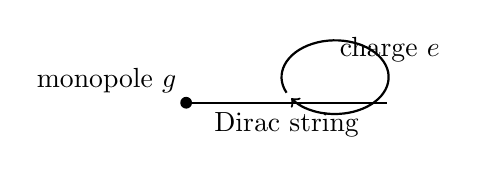
\begin{tikzpicture}[scale=0.85]
      \fill (0,0) circle (2.5pt);
      \node[above left] at (0,0) {monopole \(g\)};
      \draw[thick] (0,0) -- (3.0,0);
      \node[below] at (1.5,0) {Dirac string};
      \draw[->,thick] (1.5,0.15) arc[start angle=205,end angle=-145,
        x radius=0.8,y radius=0.55];
      \node[right] at (2.15,0.8) {charge \(e\)};
    \end{tikzpicture}
    \end{adjustbox}
    \par\smallskip\footnotesize (b) 繞弦一周的相位實驗。
  \end{minipage}
  \caption{狄拉克條件使電荷與磁荷互成反比。}
  \lectureframe{01:13:20}
  \label{fig:l04-dirac-board}
\end{figure}

若 \(e\) 很小，以電變數進行的普通微擾理論便很有用。含有更多電頂點的費曼圖會受到更強抑制。但 \eqref{eq:l04-dirac-quantization} 隨即意味著 \(g\) 很大，因此以磁頂點作圖的微擾展開並不適用。以常用的無因次耦合常數表示，
\begin{equation}
  \alpha_e=\frac{e^2}{4\pi},
  \qquad
  \alpha_m=\frac{g^2}{4\pi},
  \qquad
  \alpha_e\alpha_m=\frac{n^2}{4}.
  \label{eq:l04-dual-couplings}
\end{equation}
弱電耦合對應強磁耦合，反之亦然。

從電變數的描述來看，強耦合的磁單極子也顯得複雜。它的場能很大，周圍包覆著強烈的規範場漲落雲與虛磁荷對。它表現為沉重且延展的物件，不適合作為電變數微擾級數的起點。這不代表它比較不基本，只表示在那個物理區域中，它不是合適的初等變數。

現在想像逐漸增大 \(e\)。量子化條件迫使 \(g\) 減小。在自對偶區域附近，兩種描述都不特別弱；越過該區域後，磁變數可能變得較簡單、較輕，而電物件則受到強烈的場雲修飾。該將哪一種電荷稱為基本的，已經改變，但理論的物理內容並未改變。

\subsection{維格納之問}

希格斯玻色子究竟是基本粒子還是複合粒子的討論中，也曾出現這種模糊性。尤金·維格納一再追問「複合」到底是什麼意思。有人提出以衰變作為區分：也許基本物件不能衰變，而複合物件可以。但基態氫原子不能衰變，卻顯然是複合的；質子可能穩定而中子會衰變，但這並不表示一者是基本粒子、另一者則是原本意義下的複合粒子。每一種簡單的定義都會遇上另一個反例。

傑拉杜斯·特霍夫特最後提出一個操作性判準：若將某物件視為基本是有用的，那麼它就是基本的。這不是迴避問題，而是承認「基本」指的是能讓動力學描述簡潔的變數；而何者簡潔，可能取決於耦合與環境。

\section{走向 M 理論}

弦理論以格外鮮明的方式展現了這種角色互換。在某個參數區域，弦很輕且處於微擾區，而 D 膜則像是由弦自由度構成的沉重孤子複合物。參數改變時，D 膜可能成為較輕的基本物件；而在第一個區域中以弦描述的組態，也可以改用 D 膜來詮釋。看似基本的物件可以變成複合物；看似複合的物件也可以變成基本的。

傳統的還原論圖像暗示一條單向路徑：從大型事物一路追溯至更小的組成成分，最後抵達唯一的底層。對偶性則呈現出較不線性的圖像：耦合改變時，不同描述可以彼此轉換，沒有任何一組變數在所有情況下都占優勢。接下來將從這個角度探討 M 理論。

玻色弦的臨界維度為二十六、超弦的臨界維度為十，這些問題在此仍未解答。與其在繼續之前解決所有技術問題，我們現在轉換觀點，探討 M 理論如何在適當極限下產生弦理論。